\documentclass[12pt,a4paper]{article}

% --- Encoding / fonts / language ---
\usepackage[T1]{fontenc}
\usepackage[utf8]{inputenc}
\DeclareUnicodeCharacter{00A0}{~}
\usepackage{lmodern}
\usepackage[ngerman]{babel}
\usepackage{microtype}

% --- Graphics / links / color ---
\usepackage{graphicx}
\usepackage{hyperref}
\usepackage{xurl}
\usepackage{xcolor}
\usepackage{pdflscape}

% TikZ for diagrams from text
\usepackage{tikz}
\usetikzlibrary{arrows.meta,positioning}
\usetikzlibrary{calc,chains,shapes,fit}

\graphicspath{{diagrams/}}
\usepackage{float}

% --- Tables ---
\usepackage{array}
\usepackage{ragged2e}
\usepackage{tabularx}
\usepackage{longtable}
\usepackage{ltablex}
\keepXColumns

% --- Code / listings ---
\usepackage{listings}

% --- Page geometry ---
\usepackage{geometry}
\geometry{a4paper, top=20mm, left=20mm, right=20mm, bottom=25mm}

% --- Headers / footers ---
\usepackage{fancyhdr}
\setlength{\headheight}{15pt}
\pagestyle{fancy}
\lhead{Luca Güttinger}
\rhead{\today}
\rfoot{Seite \thepage}
\cfoot{}
\lfoot{\footnotesize\mbox{\url{https://github.com/Notenverwaltung-ch/Notenverwaltung}}}

% --- Listings config ---
\lstset{
    inputencoding=utf8,
    language=SQL,
    basicstyle=\small\ttfamily,
    breaklines=true,
    breakatwhitespace=true,
    columns=fullflexible,
    keepspaces=true,
    showstringspaces=false,
    tabsize=2,
    postbreak=\mbox{\textcolor{red}{$\hookrightarrow$}\space},
    literate={ä}{{\"a}}1 {ö}{{\"o}}1 {ü}{{\"u}}1 {Ä}{{\"A}}1 {Ö}{{\"O}}1 {Ü}{{\"U}}1 {ss}{{\ss}}1 {é}{{\'e}}1 {è}{{\`e}}1 {à}{{\`a}}1 {ê}{{\^e}}1 {ô}{{\^o}}1 {É}{{\'E}}1
}

% --- Helpers ---
\newcommand{\code}[1]{\texttt{\detokenize{#1}}}

% --- Column types for tables ---
\newcolumntype{L}[1]{>{\raggedright\arraybackslash}p{#1}}
\newcolumntype{C}[1]{>{\centering\arraybackslash}p{#1}}
\newcolumntype{R}[1]{>{\raggedleft\arraybackslash}p{#1}}
\newcolumntype{Y}{>{\raggedright\arraybackslash}X}

\setlength{\parindent}{0pt}
\setlength{\parskip}{6pt}

\setcounter{tocdepth}{4}
\setcounter{secnumdepth}{4}

\begin{document}
    \hypersetup{pageanchor=false}
% ---------------- Titelseite ----------------
    \begin{titlepage}
        \centering
        {\huge\bfseries Notenverwaltungssystem \par}
        \vspace{2cm}
        {\Large Luca Güttinger \par}
        \vspace{0.5cm}
        {\Large Dipl. Informatiker Applikationsentwicklung \par}
        \vspace{0.5cm}
        {\Large TEKO Zürich \par}
        \vspace{0.5cm}
        {\Large Datenbanken / Big Data / Data Cubes \par}
        {\Large Dozent: Milad Fakiry \par}
        \vspace{0.5cm}
        {\Large Abgabedatum: 07.09.2025 \par}
        \vfill
    \end{titlepage}
    \clearpage
    \hypersetup{pageanchor=true}
    \pagenumbering{arabic}

% ---------------- Inhaltsverzeichnis ----------------
    \tableofcontents
    \newpage

% ---------------- Einleitung ----------------


    \section{Einleitung}
    In diesem Projekt wurde ein Notenverwaltungssystem für die Website Notenverwaltung.ch entwickelt.
    Das Szenario sieht vor, dass Schülerinnen und Schüler ihre eigenen Noten jederzeit einsehen und verwalten können, auch unabhängig von Lehrpersonen.
    Zusätzlich können optionale Verwaltungsfunktionen für Fächer, Klassen, Tests und Semester genutzt werden,
    sofern diese von einer Schule oder Lehrperson bereitgestellt werden.
    Die Anwendung besteht aus einer PostgreSQL-Datenbank und einem Spring Boot Service, welcher über eine REST-API zugänglich ist.
    Die Endpunkte sind durch JWT-Token abgesichert und es existieren die Rollen \code{USER} und \code{ADMIN}.

    \subsection{Ziel der Arbeit}
    Ziel der Arbeit ist es, ein Backend für Notenverwaltung.ch zu konzipieren und umzusetzen,
    das insbesondere die eigenständige Notenverwaltung durch Schülerinnen und Schüler ermöglicht, unabhängig von Lehrpersonen. Im Fokus stehen:
    \begin{itemize}
        \item eine saubere relationale Datenbankstruktur,
        \item eine klar dokumentierte REST-API (Spring Boot) für das Erfassen, Bearbeiten und Auswerten persönlicher Leistungen,
        \item Authentifizierung und Autorisierung mittels JWT mit Rollen (\code{USER}, \code{ADMIN}),
        \item optionale Anbindung schulischer Strukturen (Fächer, Klassen, Tests, Semester), sofern verfügbar.
    \end{itemize}

    \subsection{Abgrenzung}
    Teil der Arbeit ist die Datenmodellierung, SQL-Implementierung, beispielhafte Abfragen und ein Testprotokoll.
    Ebenso wird die Absicherung der Schnittstellen (JWT) und eine rollenbasierte Zugriffskontrolle
    (\code{USER}, \code{ADMIN}) umgesetzt. Nicht Teil der Arbeit ist eine vollständige,
    produktiv eingesetzte Frontend-Weboberfläche oder die Integration in bestehende Schulinfrastrukturen; der Fokus
    liegt auf der Backend-Funktionalität für Notenverwaltung.ch. Ein eigenständiges Frontend (z. B. mit Angular) ist
    im Rahmen dieser Arbeit nicht vorgesehen oder höchstens als sehr rudimentärer Prototyp zur Veranschaulichung der API gedacht.
    \newpage

% ---------------- Anforderungsanalyse ----------------


    \section{Anforderungsanalyse}
    Im Mittelpunkt steht, dass Schülerinnen und Schüler sich registrieren bzw. anmelden, ihre persönlichen Noten sicher einsehen,
    erfassen und bei Bedarf bearbeiten sowie Auswertungen über ihre Leistungen vornehmen können.
    Lehrpersonen und Admins erhalten, soweit vorgesehen, erweiterte Funktionen zur optionalen Verwaltung von Fächern, Klassen, Tests und Semestern.
    Sicherheitsanforderungen (JWT-basierte Authentifizierung und rollenbasierte Autorisierung), Datenkonsistenz, Nachvollziehbarkeit von Änderungen
    und der Schutz personenbezogener Daten (Datensparsamkeit, Zugriff nur für Berechtigte) sind zentrale nicht‑funktionale Anforderungen.

    \subsubsection{Funktionale Anforderungen}
    \begin{itemize}
        \item Registrierung und Anmeldung von Nutzerinnen und Nutzern (USER, ADMIN).
        \item Selbstständige Verwaltung persönlicher Noten durch Benutzer: Anlegen, Bearbeiten, Löschen von Tests/Noten im eigenen Bereich.
        \item Berechnung von Durchschnittswerten und einfachen Auswertungen pro Fach/Semester.
        \item Rollenbasierter Zugriff auf REST-API-Endpunkte mit klar definierten Berechtigungen.
        \item Fehlermeldungen und Validierungen (z. B. Pflichtfelder, Wertebereiche, Dublettenprüfung bei eindeutigen Attributen).
    \end{itemize}

    \subsubsection{Nicht-funktionale Anforderungen}
    \begin{itemize}
        \item Sicherheit: JWT-basierte Authentifizierung, rollenbasierte Autorisierung, sichere Passwortspeicherung (Hashing), minimale Datenspeicherung.
        \item Datenqualität: Konsistenz durch Constraints/Referentielle Integrität, Transaktionssicherheit und Validierungen im Service.
        \item Performance und Skalierbarkeit: REST-API mit angemessenen Antwortzeiten unter typischer Last; effiziente Abfragen/Indizes.
        \item Verfügbarkeit und Betrieb: Containerisierbar (Docker), reproduzierbare lokale Entwicklung (docker-compose), einfache Deployment-Pfade.
        \item Nachvollziehbarkeit/Logging: Sinnvolle Server-Logs für Diagnose und Audit-Zwecke ohne sensible Daten im Klartext.
        \item Benutzbarkeit der API: Konsistente Endpunkte, klare Fehlercodes/-nachrichten und grundlegende Dokumentation (z. B. OpenAPI/HTTP-Beispiele).
        \item Wartbarkeit: Saubere Schichtung (Controller/Service/Repository), klare Domänenbegriffe, Tests für Kernfunktionen.
    \end{itemize}

    Die folgenden Entitäten und Beziehungen bilden diese Anforderungen im Datenmodell ab.

    Die realen Entitäten im Szenario sind:

    \begin{itemize}
        \item \textbf{Semester}: Zeitraum mit Start- und Enddatum, in dem Fächer angeboten werden.
        \item \textbf{Fach}: Lehrfach, das in Semestern angeboten wird.
        \item \textbf{Klasse}: Gruppe von Studierenden, die ein Semesterfach besuchen.
        \item \textbf{Test}: Prüfung oder Klausur, die einer Klasse zugeordnet ist.
        \item \textbf{Note}: Bewertung eines Tests für einen Studierenden.
        \item \textbf{Benutzer}: Person mit Login-Daten für das System. Kann ein Schüler, eine Lehrperson oder ein Admin sein.
        \item \textbf{Rolle}: Rollen werden als Element-Collection in \code{user_roles} ohne eigene \code{roles}-Tabelle gespeichert
        \item (\code{USER}, \code{ADMIN}).
    \end{itemize}

    \subsubsection{Beziehungen}
    \begin{itemize}
        \item Ein \textbf{Semester} hat mehrere \textbf{Semesterfächer}.
        \item Ein \textbf{Fach} kann in mehreren \textbf{Semestern} vorkommen.
        \item Ein \textbf{Semesterfach} kann mehrere \textbf{Klassen} haben.
        \item Eine \textbf{Klasse} hat mehrere \textbf{Tests}.
        \item Ein \textbf{Test} hat mehrere \textbf{Noten}.
        \item Ein \textbf{Benutzer} kann mehrere \textbf{Noten} haben.
        \item Ein \textbf{Benutzer} kann mehrere \textbf{Rollen} haben.
    \end{itemize}

% ---------------- Datenmodell ----------------
    \newpage
    \begin{landscape}
        \section{Datenmodell}

        \subsection{ER-Diagramm}
        Das folgende ER-Diagramm stellt die Entitäten, deren Attribute und die Beziehungen mit Kardinalitäten dar:

        \thispagestyle{empty}
        \begin{figure}[H]
            \centering
            \resizebox{\linewidth}{!}{
                \begin{tikzpicture}[
                    scale=1.0,
                    every node/.style={scale=1.0},
                    entity/.style={draw, rectangle, rounded corners, thick, align=left, inner sep=3pt, fill=white},
                    attr/.style={font=\scriptsize},
                    rel/.style={-Latex, thick},
                    crow/.style={-{Straight Barb[length=2.5mm]}, thick},
                    one/.style={-{}, thick},
                    note/.style={font=\scriptsize, fill=white, inner sep=1pt}
                ]
                    % Entities
                    \node[entity] (Semester) {\textbf{semesters}\\\footnotesize id: uuid (PK)\\ name: varchar(100)\\ start\_date: date\\ end\_date: date};
                    \node[entity, right=2.8cm of Semester] (Subject) {\textbf{subjects}\\\footnotesize id: uuid (PK)\\ name: varchar(150)};
                    \node[entity, below=2.0cm of $(Semester)!0.5!(Subject)$] (SemSub) {\textbf{semester\_subjects}\\\footnotesize id: uuid (PK)\\ semester\_id: uuid (FK)\\ subject\_id: uuid (FK)};
                    \node[entity, below=2.0cm of SemSub] (Class) {\textbf{classes}\\\footnotesize id: uuid (PK)\\ semester\_subject\_id: uuid (FK)\\ name: varchar(100)};
                    \node[entity, right=3.0cm of Class] (Test) {\textbf{tests}\\\footnotesize id: uuid (PK)\\ name: varchar(150)\\ class\_id: uuid (FK)\\ semester\_subject\_id: uuid (FK)\\ date: date\\ comment: varchar(1000)};
                    \node[entity, right=3.0cm of Test] (Grade) {\textbf{grades}\\\footnotesize id: uuid (PK)\\ value: numeric(4,2)\\ weight: numeric(4,2)\\ user\_id: uuid (FK)\\ test\_id: uuid (FK)\\ comment: varchar(255)};
                    \node[entity, above=1.8cm of Grade] (User) {\textbf{users}\\\footnotesize id: uuid (PK)\\ username: varchar(100)\\ password: varchar(255)\\ email: varchar(255)\\ first\_name: varchar(100)\\ last\_name: varchar(100)\\ active: boolean\\ created\_at: timestamp\\ updated\_at: timestamp};
                    \node[entity, right=2.8cm of User] (UserRole) {\textbf{user\_roles}\\\footnotesize user\_id: uuid (FK)\\ role: varchar(50)};

                    % Relationships
                    \draw[rel] (Semester) -- node[pos=0.05, above, note]{1} node[pos=0.95, above, note]{m} (SemSub);
                    \draw[rel] (Subject) -- node[pos=0.05, above, note]{1} node[pos=0.95, above, note]{m} (SemSub);
                    \draw[rel] (SemSub) -- node[pos=0.1, left, note]{1} node[pos=0.9, left, note]{m} (Class);
                    \draw[rel] (Class) -- node[pos=0.05, above, note]{1} node[pos=0.95, above, note]{m} (Test);
                    \draw[rel] (Test) -- node[pos=0.05, above, note]{1} node[pos=0.95, above, note]{m} (Grade);
                    \draw[rel] (User) -- node[pos=0.05, right, note]{1} node[pos=0.95, right, note]{m} (Grade);
                    \draw[rel] (User) -- node[pos=0.05, above, note]{1} node[pos=0.95, above, note]{m} (UserRole);
                \end{tikzpicture}
            }
            \caption{ER-Diagramm des Notenverwaltungssystems}
            \label{fig:erd}
        \end{figure}
    \end{landscape}

    \subsection{Tabellenbeschreibung}
    Im Folgenden werden die Tabellen detailliert beschrieben. Für jede Entität gibt es eine separate Tabelle mit Attributen, Datentypen, Pflichten und Schlüsseln.

    \subsubsection{semesters}
    \begin{longtable}{|L{4cm}|L{3cm}|L{3cm}|L{4cm}|}
        \hline
        \textbf{Attribut} & \textbf{Datentyp} & \textbf{Pflicht} & \textbf{Bemerkung} \\ \hline
        id & uuid & ja & Primärschlüssel \\ \hline
        name & varchar(100) & ja & z. B. HS2025 \\ \hline
        start\_date & date & ja &  \\ \hline
        end\_date & date & ja &  \\ \hline
    \end{longtable}
    \textbf{Schlüssel / Constraints:} PK: id

    \subsubsection{subjects}
    \begin{longtable}{|L{4cm}|L{3cm}|L{3cm}|L{4cm}|}
        \hline
        \textbf{Attribut} & \textbf{Datentyp} & \textbf{Pflicht} & \textbf{Bemerkung} \\ \hline
        id & uuid & ja & Primärschlüssel \\ \hline
        name & varchar(150) & ja & Eindeutig (Unique) empfohlen \\ \hline
    \end{longtable}
    \textbf{Schlüssel / Constraints:} PK: id

    \subsubsection{semester\_subjects}
    \begin{longtable}{|L{4cm}|L{3cm}|L{3cm}|L{4cm}|}
        \hline
        \textbf{Attribut} & \textbf{Datentyp} & \textbf{Pflicht} & \textbf{Bemerkung} \\ \hline
        id & uuid & ja & Primärschlüssel \\ \hline
        semester\_id & uuid & ja & FK $\rightarrow$ semesters(id) \\ \hline
        subject\_id & uuid & ja & FK $\rightarrow$ subjects(id) \\ \hline
    \end{longtable}
    \textbf{Schlüssel / Constraints:} PK: id; Unique(semester\_id, subject\_id) empfohlen

    \subsubsection{classes}
    \begin{longtable}{|L{4cm}|L{3cm}|L{3cm}|L{4cm}|}
        \hline
        \textbf{Attribut} & \textbf{Datentyp} & \textbf{Pflicht} & \textbf{Bemerkung} \\ \hline
        id & uuid & ja & Primärschlüssel \\ \hline
        semester\_subject\_id & uuid & ja & FK $\rightarrow$ semester\_subjects(id) \\ \hline
        name & varchar(100) & nein & optionale Klassenbezeichnung \\ \hline
    \end{longtable}
    \textbf{Schlüssel / Constraints:} PK: id; FK: semester\_subject\_id

    \subsubsection{tests}
    \begin{longtable}{|L{4cm}|L{3cm}|L{3cm}|L{4cm}|}
        \hline
        \textbf{Attribut} & \textbf{Datentyp} & \textbf{Pflicht} & \textbf{Bemerkung} \\ \hline
        id & uuid & ja & Primärschlüssel \\ \hline
        name & varchar(150) & ja &  \\ \hline
        class\_id & uuid & ja & FK $\rightarrow$ classes(id) \\ \hline
        semester\_subject\_id & uuid & ja & FK $\rightarrow$ semester\_subjects(id) \\ \hline
        date & date & ja & Datum des Tests (liegt im Idealfall im Semesterzeitraum) \\ \hline
        comment & varchar(1000) & nein & Freitext, optionaler Kommentar zum Test \\ \hline
    \end{longtable}
    \textbf{Schlüssel / Constraints:} PK: id; FK: class\_id; FK: semester\_subject\_id

    \subsubsection{grades}
    \begin{longtable}{|L{4cm}|L{3cm}|L{3cm}|L{4cm}|}
        \hline
        \textbf{Attribut} & \textbf{Datentyp} & \textbf{Pflicht} & \textbf{Bemerkung} \\ \hline
        id & uuid & ja & Primärschlüssel \\ \hline
        value & numeric(4,2) & ja & Notenwert (z. B. 1.0-6.0) \\ \hline
        weight & numeric(4,2) & ja & Gewichtung in Prozent \\ \hline
        student\_id & uuid & ja & FK $\rightarrow$ users(id) \\ \hline
        test\_id & uuid & nein & FK $\rightarrow$ tests(id) \\ \hline
        comment & varchar(255) & nein & Freitext \\ \hline
    \end{longtable}
    \textbf{Schlüssel / Constraints:} PK: id; FK: student\_id; FK: test\_id; Unique(student\_id, test\_id) empfohlen

    \subsubsection{users}
    \begin{longtable}{|L{4cm}|L{3cm}|L{3cm}|L{4cm}|}
        \hline
        \textbf{Attribut} & \textbf{Datentyp} & \textbf{Pflicht} & \textbf{Bemerkung} \\ \hline
        id & uuid & ja & Primärschlüssel \\ \hline
        username & varchar(100) & ja & Eindeutig (Unique) \\ \hline
        password & varchar(255) & ja & Hash (BCrypt) \\ \hline
        email & varchar(255) & nein & Eindeutig (Unique) empfohlen \\ \hline
        first\_name & varchar(100) & nein &  \\ \hline
        last\_name & varchar(100) & nein &  \\ \hline
        date\_of\_birth & date & nein &  \\ \hline
        active & boolean & ja & Default: false \\ \hline
        created\_at & timestamp & ja &  \\ \hline
        updated\_at & timestamp & nein &  \\ \hline
    \end{longtable}
    \textbf{Schlüssel / Constraints:} PK: id

    \subsubsection{user\_roles}
    \begin{longtable}{|L{4cm}|L{3cm}|L{3cm}|L{4cm}|}
        \hline
        \textbf{Attribut} & \textbf{Datentyp} & \textbf{Pflicht} & \textbf{Bemerkung} \\ \hline
        user\_id & uuid & ja & FK $\rightarrow$ users(id) \\ \hline
        role & varchar(50) & ja & z. B. ADMIN, USER \\ \hline
    \end{longtable}
    \textbf{Schlüssel / Constraints:} PK: (user\_id, role); FK: user\_id

% ---------------- Umsetzungsbeschreibung ----------------


    \section{Umsetzungsbeschreibung}

    Die Notenverwaltung ist als Spring Boot Service realisiert und stellt eine REST-API zur Verfügung. Persistenz wird über JPA/Hibernate umgesetzt. Die Authentifizierung
    und Autorisierung erfolgen über Spring Security mit JWTs und rollenbasierten Berechtigungen
    (\code{USER}, \code{ADMIN}). Eine OpenAPI/Swagger-Dokumentation beschreibt die Schnittstellen.

    \subsection{Architektur \/ Spring Boot Service}
    Die Anwendung ist als monolithischer Spring Boot Service aufgebaut und folgt einer klaren Schichtentrennung:
    \begin{itemize}
        \item \textbf{Controller-Schicht}: REST-Endpoints (z. B. \code{/api/public/auth}, \code{/api/subjects})
        \item \textbf{Service-Schicht}: Kapselt Geschäftslogik, Transaktionen und Validierungen; orchestriert Zugriffe auf Repositories.
        \item \textbf{Repository-Schicht}: Spring Data JPA Repositories für CRUD-Operationen und abgeleitete/annotierte Queries.
        \item \textbf{Domain\/Model}: JPA-Entities (z. B. \code{Semester}, \code{Subject}, \code{Class}, \code{Test}, \code{Grade}, \code{User}) sowie eine Element-Collection \code{user_roles} für Rollen (keine separate \code{roles}-Tabelle).
    \end{itemize}
    Der Service ist containerisierbar (Docker) und wird in der lokalen Entwicklung via \code{docker-compose} mit PostgreSQL betrieben.

    \subsection{Persistenz mit JPA\/Hibernate}
    Die Persistenzschicht verwendet Spring Data JPA mit Hibernate als Implementierung. Entities sind mit JPA-Annotationen versehen
    (z. B. \code{@Entity}, \code{@Table}, \code{@Id}, \code{@ManyToOne}, \code{@OneToMany}). Repositories werden als Interfaces
    (\code{extends JpaRepository<..., ...>}) definiert und liefern Standard-CRUD sowie abgeleitete Finder
    (z. B. \code{findByName}, \code{findByUserIdAndTestId}).\newline
    Transaktionen werden deklarativ über \code{@Transactional} (Service-Schicht) gesteuert.
    Datenintegrität wird sowohl über DB-Constraints (PK, FK, Unique) als auch über Bean Validation (z. B. \code{@NotNull},
    \code{@Size}) sichergestellt.

    \subsection{Sicherheit: Spring Security mit JWT}
    Die API ist über JWT gesichert. Der typische Flow:
    \begin{enumerate}
        \item Nutzer meldet sich über \code{POST /api/auth/login} mit Benutzername / Passwort an.
        \item Bei Erfolg wird ein signiertes JWT (inkl. Rollen-Claims) ausgestellt und im Client gespeichert.
        \item Folgeaufrufe enthalten \code{Authorization: Bearer <token>}; die Security-Konfiguration prüft Signatur, Gültigkeit und Rollen.
    \end{enumerate}
    Rollenbasierte Autorisierung wird per Ant-Matcher / Methodensicherheit \newline
    (z.B. \code{@PreAuthorize("hasRole('ADMIN')")}) umgesetzt.
    Passwörter werden mit BCrypt gehasht.

    \subsection{OpenAPI / Swagger}
    Die REST-Schnittstellen sind mit OpenAPI beschrieben. Während der Entwicklung ist die UI unter \code{/api/public/docs} erreichbar.
    Die Spezifikation (JSON / YAML) ermöglicht die Generierung von Clients und dient der API-Dokumentation.
    Endpunkte, Request / Response-Schemata sowie Fehlercodes sind dort ersichtlich. Die Swagger Dokumentation ist im Ordner \code{documentation/swagger} abgelegt.

% ---------------- SQL-Implementierung ----------------

    \subsection{SQL-Implementierung}
    In dieser Anwendung wird das Datenbankschema strikt mittels Flyway-Migrationen versioniert und aufgebaut.
    Die DDL (CREATE TABLE, Constraints, Indizes) wird also über SQL-Skripte in den Flyway-Migrationsdateien gepflegt.
    Dagegen sind die nachfolgenden INSERT- und SELECT-Beispiele als illustrative, vereinfachte SQLs zu verstehen:
    In der produktiven Anwendung werden entsprechende Datenzugriffe hauptsächlich über Spring Data JPA Repositories
    umgesetzt und nicht 1:1 mit diesen Roh-SQLs ausgeführt.

    \subsubsection{Schema-Definitionen}

    Die folgenden Ausschnitte zeigen Auszüge aus der initialen Flyway-Migration. Weitere CREATE-Statements (inkl. Constraints)
    befinden sich vollständig in folgendem Ordner: \\
    \code{src/main/resources/db/migration}.

    \lstinputlisting[language=SQL]{sql/schema_excerpt.sql}

    \subsubsection{Beispielhafte INSERT-Befehle}
    \noindent Die folgenden Inserts legen einige Beispiel-Datensätze an. Jede Gruppe ist nach Tabelle sortiert und kurz kommentiert.
    \lstinputlisting[language=SQL]{sql/inserts_examples.sql}

    \textit{Erläuterung:}
    \begin{itemize}
        \item Users: Erstellt zwei Demo-Benutzer (Studierende), um Join-Abfragen zu veranschaulichen.
        \item Subjects: Fügt die Fächer hinzu, die in HS2025 angeboten werden.
        \item Semesters: Definiert den Zeitraum HS2025, auf den die anderen Daten referenzieren.
        \item Semester\_Subjects: Verknüpft Semester und Fächer und bildet das Lehrangebot ab.
        \item Classes: Legt je eine Klasse pro Fach im Semester HS2025 an.
        \item Tests: Erzeugt pro Klasse einen Test mit Datum und Maximalpunkten.
        \item Grades: Vergibt zwei Noten für die beiden Studierenden auf die Tests.
    \end{itemize}

% ---------------- Beispielabfragen ----------------

    \subsubsection{Beispielhafte SELECT-Befehle}
    Die folgenden SELECT-Beispiele sind didaktisch und werden in der Anwendung so nicht direkt ausgeführt. In der Praxis übernimmt die Repository-Schicht (Spring Data JPA) die Abfragen.
    \lstinputlisting[language=SQL]{sql/selects_examples.sql}

    \subsubsection{Beispielhafte Hibernate Query}
    Abschliessend ein konkretes Beispiel, wie eine solche Abfrage in der Anwendung über ein Repository umgesetzt ist.
    Die Methode liefert die Noten eines Semesters (optional gefiltert nach Student) als DTO:
    \begin{lstlisting}[language=Java]
    @Query("select new ch.notenverwaltung.model.dto.SemesterGradeRow(" +
            " g.id, u.id, u.firstName, u.lastName, subj.id, subj.name, t.id, t.name, t.date, g.value, g.weight, g.comment) " +
            " from Grade g " +
            " join g.student u " +
            " left join g.test t " +
            " left join t.semesterSubject ss " +
            " left join ss.subject subj " +
            " left join ss.semester sem " +
            " where sem.id = :semesterId " +
            " and ( u.id = COALESCE(:studentId, u.id) )")
    List<SemesterGradeRow> findSemesterGrades(@Param("semesterId") UUID semesterId,
                                              @Param("studentId") UUID studentId);
    \end{lstlisting}

    \textbf{Beispielausgabe (Auszug):}\\
    \begin{figure}[H]
        \centering
        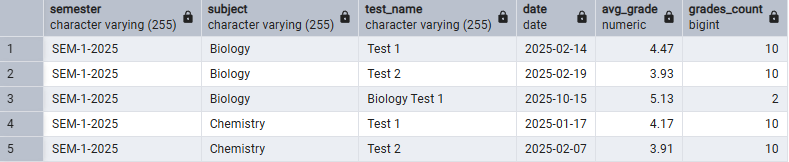
\includegraphics[width=0.95\linewidth]{images/sql_output_3}
        \caption{Beispielausgabe: 3: Alle Tests eines Semesters mit Durchschnittsnote pro Test}
        \label{fig:sql_output_3}
    \end{figure}
    \begin{figure}[H]
        \centering
        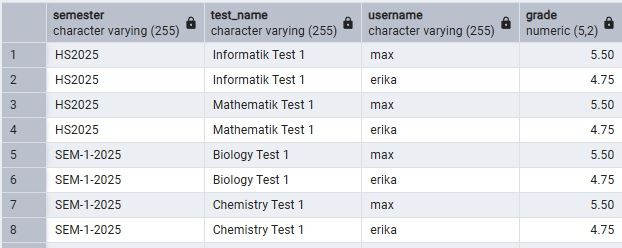
\includegraphics[width=0.95\linewidth]{images/sql_output_6}
        \caption{Beispielausgabe: 6. Rangliste pro Test (beste zuerst) inkl. Semester}
        \label{fig:sql_output_6}
    \end{figure}
    \begin{figure}[H]
        \centering
        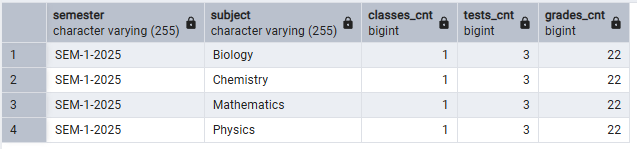
\includegraphics[width=0.95\linewidth]{images/sql_output_7}
        \caption{Beispielausgabe: 7: Workload je Fach im Semester: Anzahl Klassen, Tests, Bewertungen}
        \label{fig:sql_output_7}
    \end{figure}
    \newpage

% ---------------- Testprotokoll ----------------


    \section{Testprotokoll}

    \subsection{Beschreibung}
    Die Tests wurden sowohl mit manuellen SQL-Abfragen als auch über die REST-API (gesichert durch JWT) durchgeführt.

    \subsection{Testfälle}\label{sec:testfaelle}

    \subsubsection{T1 - User anlegen (gültige Daten)}
    \begin{small}
        \begin{tabularx}{\textwidth}{|L{3.2cm}|Y|}
            \hline
            \textbf{Feld} & \textbf{Wert} \\ \hline
            ID & T1 \\ \hline
            Erwartet & User wird gespeichert \\ \hline
            Status & Pass \\ \hline
            Datum/Tester & 2025-09-04 / Luca G. \\ \hline
            ENV & DEV (Docker, Postgres 16, SB 3.3) \\ \hline
            Pre-Conditions & Admin-Token vorhanden; Username noch nicht vergeben \\ \hline
            Endpoint/Schritte & \code{POST /api/admin/users} mit Body \code{\{username, password, roles:[\"USER\"]\}} \\ \hline
            Response (gekürzt) & \code{201 Created}; JSON mit \code{id, username, roles, active, created_at} \\ \hline
            Post-Conditions & User existiert in Tabelle \code{users}; Auditfelder gesetzt \\ \hline
            Referenz & REQ-USR-001 \\ \hline
        \end{tabularx}
    \end{small}

    \subsubsection{T2 - User anlegen (fehlende Pflichtfelder)}
    \begin{small}
        \begin{tabularx}{\textwidth}{|L{3.2cm}|Y|}
            \hline
            \textbf{Feld} & \textbf{Wert} \\ \hline
            ID & T2 \\ \hline
            Erwartet & HTTP 400 Validierung \\ \hline
            Status & Pass \\ \hline
            Datum/Tester & 2025-09-04 / Luca G. \\ \hline
            ENV & DEV \\ \hline
            Pre-Conditions & Admin-Token vorhanden \\ \hline
            Endpoint/Schritte & \code{POST /api/admin/users} (ungültiger Body) \\ \hline
            Response (gekürzt) & \code{400 Bad Request} mit Validierungsfehlern \\ \hline
            Post-Conditions & Kein Datensatz angelegt \\ \hline
            Referenz & REQ-USR-002 \\ \hline
        \end{tabularx}
    \end{small}

    \subsubsection{T3 - Semester hinzufügen}
    \begin{small}
        \begin{tabularx}{\textwidth}{|L{3.2cm}|Y|}
            \hline
            \textbf{Feld} & \textbf{Wert} \\ \hline
            ID & T3 \\ \hline
            Erwartet & In Liste sichtbar \\ \hline
            Status & Pass \\ \hline
            Datum/Tester & 2025-09-04 / Luca G. \\ \hline
            ENV & DEV \\ \hline
            Pre-Conditions & Admin-Token vorhanden \\ \hline
            Endpoint/Schritte & \code{INSERT}/\code{POST} Semester $\rightarrow$ anschliessend \code{GET /api/semesters} \\ \hline
            Response (gekürzt) & \code{201 Created}; Objekt in GET-Liste vorhanden \\ \hline
            Post-Conditions & Semester existiert \\ \hline
            Referenz & REQ-SEM-001 \\ \hline
        \end{tabularx}
    \end{small}

    \subsubsection{T4 - Subject anlegen (Duplicate Name)}
    \begin{small}
        \begin{tabularx}{\textwidth}{|L{3.2cm}|Y|}
            \hline
            \textbf{Feld} & \textbf{Wert} \\ \hline
            ID & T4 \\ \hline
            Erwartet & 409/400 Konflikt bei doppeltem Namen \\ \hline
            Status & Pass \\ \hline
            Datum/Tester & 2025-09-04 / Luca G. \\ \hline
            ENV & DEV \\ \hline
            Pre-Conditions & Admin-Token vorhanden und Subject mit \code{name=Mathematik} existiert bereits \\ \hline
            Endpoint/Schritte & \code{POST /api/subjects} mit Body \code{\{name:"Mathematik"\}} \\ \hline
            Response (gekürzt) & \code{409 Conflict} oder \code{400 Bad Request} mit Fehlermeldung \\ \hline
            Post-Conditions & Kein weiteres Subject mit gleichem Namen \\ \hline
            Referenz & REQ-SUB-002 \\ \hline
        \end{tabularx}
    \end{small}

    \subsubsection{T5 - SemesterSubject Zuordnung}
    \begin{small}
        \begin{tabularx}{\textwidth}{|L{3.2cm}|Y|}
            \hline
            \textbf{Feld} & \textbf{Wert} \\ \hline
            ID & T5 \\ \hline
            Erwartet & Kombination Semester+Subject wird angelegt \\ \hline
            Status & Pass \\ \hline
            Datum/Tester & 2025-09-04 / Luca G. \\ \hline
            ENV & DEV \\ \hline
            Pre-Conditions & Admin-Token vorhanden und Semester \code{HS2025} und Subject \code{Mathematik} existieren \\ \hline
            Endpoint/Schritte & \code{POST /api/semester-subjects} mit \code{\{semesterId, subjectId\}} \\ \hline
            Response (gekürzt) & \code{201 Created}; Objekt enth\"alt IDs \\ \hline
            Post-Conditions & Datensatz in \code{semester_subjects} existiert \\ \hline
            Referenz & REQ-SS-001 \\ \hline
        \end{tabularx}
    \end{small}

    \subsubsection{T6 - SemesterSubject doppelt}
    \begin{small}
        \begin{tabularx}{\textwidth}{|L{3.2cm}|Y|}
            \hline
            \textbf{Feld} & \textbf{Wert} \\ \hline
            ID & T6 \\ \hline
            Erwartet & Unique verhindert Duplikat \\ \hline
            Status & Pass \\ \hline
            Datum/Tester & 2025-09-04 / Luca G. \\ \hline
            ENV & DEV \\ \hline
            Pre-Conditions & Admin-Token vorhanden und Zuordnung Semester \code{HS2025} + \code{Mathematik} existiert \\ \hline
            Endpoint/Schritte & Erneuter \code{POST /api/semester-subjects} mit derselben Kombination \\ \hline
            Response (gekürzt) & \code{409 Conflict} oder \code{400} mit Unique-Fehler \\ \hline
            Post-Conditions & Kein zweiter Datensatz angelegt \\ \hline
            Referenz & REQ-SS-002 \\ \hline
        \end{tabularx}
    \end{small}

    \subsubsection{T7 - Klasse zu SemesterSubject}
    \begin{small}
        \begin{tabularx}{\textwidth}{|L{3.2cm}|Y|}
            \hline
            \textbf{Feld} & \textbf{Wert} \\ \hline
            ID & T7 \\ \hline
            Erwartet & Klasse referenziert gültiges SemesterSubject \\ \hline
            Status & Pass \\ \hline
            Datum/Tester & 2025-09-04 / Luca G. \\ \hline
            ENV & DEV \\ \hline
            Pre-Conditions & Admin-Token vorhanden und \code{semester_subjects}-Datensatz vorhanden \\ \hline
            Endpoint/Schritte & \code{POST /api/classes} mit \code{\{semesterSubjectId, name\}} \\ \hline
            Response (gekürzt) & \code{201 Created}; Klasse enth\"alt \code{semesterSubjectId} \\ \hline
            Post-Conditions & Datensatz in \code{classes} existiert \\ \hline
            Referenz & REQ-CLS-001 \\ \hline
        \end{tabularx}
    \end{small}

    \subsubsection{T8 - Test an Klasse anlegen}
    \begin{small}
        \begin{tabularx}{\textwidth}{|L{3.2cm}|Y|}
            \hline
            \textbf{Feld} & \textbf{Wert} \\ \hline
            ID & T8 \\ \hline
            Erwartet & Test referenziert korrekt Klasse und SemesterSubject \\ \hline
            Status & Pass \\ \hline
            Datum/Tester & 2025-09-04 / Luca G. \\ \hline
            ENV & DEV \\ \hline
            Pre-Conditions & Admin-Token vorhanden und Klasse existiert \\ \hline
            Endpoint/Schritte & \code{POST /api/tests} mit \code{\{classId, semesterSubjectId, name, date\}} \\ \hline
            Response (gekürzt) & \code{201 Created}; Test enth\"alt \code{classId, semesterSubjectId} \\ \hline
            Post-Conditions & Datensatz in \code{tests} existiert \\ \hline
            Referenz & REQ-TST-001 \\ \hline
        \end{tabularx}
    \end{small}

    \subsubsection{T9 - Note für Student+Test}
    \begin{small}
        \begin{tabularx}{\textwidth}{|L{3.2cm}|Y|}
            \hline
            \textbf{Feld} & \textbf{Wert} \\ \hline
            ID & T9 \\ \hline
            Erwartet & Ein Datensatz in \code{grades} \\ \hline
            Status & Pass \\ \hline
            Datum/Tester & 2025-09-04 / Luca G. \\ \hline
            ENV & DEV \\ \hline
            Pre-Conditions & Admin-Token vorhanden und Test und User existieren \\ \hline
            Endpoint/Schritte & \code{POST /api/grades} mit \code{\{userId, testId, value\}} \\ \hline
            Response (gekürzt) & \code{201 Created}; Grade enth\"alt \code{userId, testId, value} \\ \hline
            Post-Conditions & Datensatz in \code{grades} existiert \\ \hline
            Referenz & REQ-GRD-001 \\ \hline
        \end{tabularx}
    \end{small}

    \subsubsection{T10 - Note doppelt gleicher Student+Test}
    \begin{small}
        \begin{tabularx}{\textwidth}{|L{3.2cm}|Y|}
            \hline
            \textbf{Feld} & \textbf{Wert} \\ \hline
            ID & T10 \\ \hline
            Erwartet & Duplikat wird verhindert \\ \hline
            Status & Pass \\ \hline
            Datum/Tester & 2025-09-04 / Luca G. \\ \hline
            ENV & DEV \\ \hline
            Pre-Conditions & Admin-Token vorhanden und Grade für (\code{userId}, \code{testId}) existiert bereits \\ \hline
            Endpoint/Schritte & Erneuter \code{POST /api/grades} mit gleichem \code{userId+testId} \\ \hline
            Response (gekürzt) & \code{409 Conflict} oder \code{400} mit Unique-Fehlermeldung \\ \hline
            Post-Conditions & Kein zweiter Datensatz für gleiche Kombination \\ \hline
            Referenz & REQ-GRD-002 \\ \hline
        \end{tabularx}
    \end{small}

    \subsubsection{T11 - JWT mit gültigem Token}
    \begin{small}
        \begin{tabularx}{\textwidth}{|L{3.2cm}|Y|}
            \hline
            \textbf{Feld} & \textbf{Wert} \\ \hline
            ID & T11 \\ \hline
            Erwartet & Zugriff erlaubt (\code{HTTP 200}) \\ \hline
            Status & Pass \\ \hline
            Datum/Tester & 2025-09-04 / Luca G. \\ \hline
            ENV & DEV \\ \hline
            Pre-Conditions & Admin-Token vorhanden \\ \hline
            Endpoint/Schritte & \code{GET /api/semesters} mit \code{Authorization: Bearer <token>} \\ \hline
            Response (gekürzt) & \code{200 OK}; Seite mit Semestern \\ \hline
            Post-Conditions & Keine Änderungen an Daten \\ \hline
            Referenz & SEC-AUTH-001 \\ \hline
        \end{tabularx}
    \end{small}

    \subsubsection{T12 - Zugriff ohne Token}
    \begin{small}
        \begin{tabularx}{\textwidth}{|L{3.2cm}|Y|}
            \hline
            \textbf{Feld} & \textbf{Wert} \\ \hline
            ID & T12 \\ \hline
            Erwartet & 401 verweigert \\ \hline
            Status & Pass \\ \hline
            Datum/Tester & 2025-09-04 / Luca G. \\ \hline
            ENV & DEV \\ \hline
            Pre-Conditions & Kein \code{Authorization} Header \\ \hline
            Endpoint/Schritte & \code{GET /api/semesters} ohne Token \\ \hline
            Response (gekürzt) & \code{401 Unauthorized} \\ \hline
            Post-Conditions & Keine Änderungen an Daten \\ \hline
            Referenz & SEC-AUTH-002 \\ \hline
        \end{tabularx}
    \end{small}

    \subsubsection{T13 - Rolle unzureichend}
    \begin{small}
        \begin{tabularx}{\textwidth}{|L{3.2cm}|Y|}
            \hline
            \textbf{Feld} & \textbf{Wert} \\ \hline
            ID & T13 \\ \hline
            Erwartet & 403 verweigert \\ \hline
            Status & Pass \\ \hline
            Datum/Tester & 2025-09-04 / Luca G. \\ \hline
            ENV & DEV \\ \hline
            Pre-Conditions & Benutzer mit \code{ROLE_USER} ohne Adminrechte \\ \hline
            Endpoint/Schritte & \code{POST /api/semesters} mit \code{ROLE_USER} \\ \hline
            Response (gekürzt) & \code{403 Forbidden} \\ \hline
            Post-Conditions & Kein Datensatz angelegt \\ \hline
            Referenz & SEC-AUTH-003 \\ \hline
        \end{tabularx}
    \end{small}

    \subsubsection{T14 - Paging/Filter Grades}
    \begin{small}
        \begin{tabularx}{\textwidth}{|L{3.2cm}|Y|}
            \hline
            \textbf{Feld} & \textbf{Wert} \\ \hline
            ID & T14 \\ \hline
            Erwartet & Korrekte Anzahl und Filterung der Ergebnisse \\ \hline
            Status & Pass \\ \hline
            Datum/Tester & 2025-09-04 / Luca G. \\ \hline
            ENV & DEV \\ \hline
            Pre-Conditions & Mehrere \code{grades} im System \\ \hline
            Endpoint/Schritte & \code{GET /api/grades?page=0\&size=10\&valueMin=4.0} \\ \hline
            Response (gekürzt) & \code{200 OK}; Page mit erwarteter Anzahl und Filter \\ \hline
            Post-Conditions & Keine Änderungen an Daten \\ \hline
            Referenz & REQ-GRD-003 \\ \hline
        \end{tabularx}
    \end{small}

    \subsubsection{T15 - Subject löschen mit Referenzen}
    \begin{small}
        \begin{tabularx}{\textwidth}{|L{3.2cm}|Y|}
            \hline
            \textbf{Feld} & \textbf{Wert} \\ \hline
            ID & T15 \\ \hline
            Erwartet & Löschen gemäss Policy verhindert (FK) \\ \hline
            Status & Pass \\ \hline
            Datum/Tester & 2025-09-04 / Luca G. \\ \hline
            ENV & DEV \\ \hline
            Pre-Conditions & Subject ist referenziert (\code{semester_subjects}/\code{classes}/\code{tests}) \\ \hline
            Endpoint/Schritte & \code{DELETE /api/subjects/\{id\}} \\ \hline
            Response (gekürzt) & \code{409 Conflict} oder Fehlermeldung zur referenziellen Integrität \\ \hline
            Post-Conditions & Subject bleibt bestehen; oder Cascade gemäss definierter Policy \\ \hline
            Referenz & REQ-SUB-003 \\ \hline
        \end{tabularx}
    \end{small}

    \subsection{Testdaten}
    In diesem Repository stehen zwei HTTP-Dateien zur Verf\"ugung, mit denen sich die Testdaten einfach vorbereiten und alle
    Testf\"alle ausf\"uhren lassen: \code{documentation/testcases}.\newline
    F\"uhre zun\"achst \code{testdata-setup.http} aus, um die Basisdaten (z.\,B. Semester, Subject, Zuordnung, Klasse, Test)
    anzulegen; anschliessend k\"onnen die einzelnen Testf\"alle direkt \"uber \code{testcase.http} gegen die laufende Anwendung
    ausgef\"uhrt werden.\newline
    Die Requests sind so vorbereitet, dass sie mit dem JetBrains HTTP Client (IDE) sofort lauff\"ahig sind und Token/IDs automatisch
    in der Session hinterlegt werden.


    \newpage

% ---------------- Fazit ----------------


    \section{Fazit \& Reflexion}
    Das Projekt hat gezeigt, wie eine relationale Datenbank modelliert und umgesetzt werden kann.
    Gut funktioniert hat die Modellierung der Entitäten und die Umsetzung der REST-API.
    Herausfordernd war die korrekte Abbildung der Beziehungen zwischen Tests, Klassen und Semestern.

    Aus persönlicher Sicht konnte ich insbesondere auf bereits vorhandene Erfahrung mit Spring und
    dem Aufbau von Datenbank-Services (Repository/Service-Layer, Transaktionen, JPA-Mapping,
    Paging/Sorting) zurückgreifen. Dadurch ging die Implementierung der grundlegenden CRUD-Funktionen
    und der fachlichen Services effizient voran.

    Besonders spannend war für mich, mich vertieft in die Security-Themen von Spring einzuarbeiten.
    Dazu gehörten unter anderem die Konfiguration von SecurityFilterChain, die Definition von
    rollenbasierten Berechtigungen (Method Security/Endpoint Security) sowie das Verständnis für
    Authentifizierungs- und Autorisierungsflüsse (z. B. Bearer Token/JWT). Diese Aspekte haben mein
    Verständnis für sichere API-Designs deutlich erweitert und werden meine zukünftigen Projekte
    nachhaltig prägen.

    Ein weiterer Fokus lag auf der korrekten Verwendung von Swagger/OpenAPI. Neben der Generierung
    einer konsistenten API-Dokumentation habe ich Wert darauf gelegt, sinnvolle Schemas, Beispiele
    und Response-Codes zu hinterlegen, damit die Schnittstellen für Konsumentinnen und Konsumenten
    klar und testbar sind. Die Integration der Swagger-UI erleichtert dabei sowohl die manuelle
    Verifikation einzelner Endpunkte als auch die Kommunikation im Team.

    Insgesamt hat das Projekt meine Stärken im Bereich Spring und Datenbank-Services bestätigt und
    gleichzeitig meinen Werkzeugkasten um wichtige Security- und Dokumentations-Bausteine erweitert.

    Rückblickend war es zudem spannend, die gesamte Dokumentation mit \LaTeX{} zu erstellen. Die klare
    Trennung von Inhalt und Formatierung, die sauberen Querverweise sowie die gute Unterstützung für
    Code-Listings und Tabellen haben zu einer einheitlichen Ausarbeitung beigetragen.

    Ein weiterer wichtiger Punkt war die Erstellung der CI/CD-Pipeline zur automatischen PDF-Generierung.
    Diese Phase war zuweilen recht anstrengend: Von der korrekten Einrichtung der \LaTeX{}-Toolchain in
    der Build-Umgebung über Paketabhängigkeiten bis hin zu Pfad- und Encoding-Themen gab es einige
    Hürden. Nachdem alle Stolpersteine beseitigt waren, konnte die Pipeline schliesslich zuverlässig die
    PDF-Dokumentation bauen – ein Ergebnis, das den Aufwand nachhaltig rechtfertigt und die Wartbarkeit
    in Zukunft deutlich verbessert.
% ---------------- Anhang ----------------

    \newpage


    \section{Anhang}

    \subsection{SQL-Dump}
    Der vollständige SQL-Dump befindet sich im Ordner \code{documentation/dump} dieses Repositories
    (\code{documentation/dump/backup_nv_final.sql}).\newline
    Der Dump wurde mit folgendem Befehl erstellt:
    \begin{lstlisting}[language=bash]
pg_dump -h localhost -p 5432 -U postgres -d notenverwaltung -F p -f documentation/dump/backup_nv_final.sql
    \end{lstlisting}

    \subsubsection{SQL Schema}
    Das vollständige CREATE-Skript (Flyway Migrationen) ist im Ordner\\ \code{src/main/resources/db/migration/} zu finden.

    \subsection{OpenAPI Dokumentation}
    Die vollständige OpenAPI/Swagger-Dokumentation der REST-API befindet sich im Ordner \code{documentation/swagger/documentation.json}.
    Swagger-UI ist unter \code{/api/public/docs} erreichbar.

    \subsection{Sourcecode und Release}
    Der komplette Sourcecode ist öffentlich auf GitHub unter:\\
    \url{https://github.com/Notenverwaltung-ch/Notenverwaltung}

    In der finalen Abgabe liegt zusätzlich eine ZIP-Datei bei, die den vollständigen Sourcecode enthält.\\
    Alternativ steht ein Release zum Download bereit:
    \href{https://github.com/Notenverwaltung-ch/Notenverwaltung/releases/tag/25.1.0}{Release 25.1.0}

    \subsection{Testfälle aus dem Testprotokoll}
    Die HTTP Files um die Testfälle aus dem Testprotokoll ausführen zu können befinden sich im Ordner \code{documentation/testcases} dieses Repositories.

\end{document}
